\chapter{Bridging the Gap}\label{chapter:solutions}

In the previous chapters, I explored the history of machine learning and provided a comprehensive overview of the most critical aspects of the \ac{MLOps} life cycle, and briefly discussed the reasons for why the gap between running code locally on developer's machine and deploying it in a cloud-based environment for running.
\newline
This chapter aims to introduce strategies for overcoming this gap and its associated challanges. Integrating these strategies requires a comprehensive understanding of both the theoretical and practical aspects of cloud computing and local development environments. It is important to point out that each strategy outlined in this chapter is accompanied by a comprehensive explanation of how it works, and include code examples that demonstrate its practical application.
\section{Containerization}
In order to grasp the concept of containerization, it is essential to understand the concept of vertualization and the differences between various virtualization mechanisms.

\subsection{Virtualization}
Virtualization is the process of creating a virtual version or several virtual versions of a piece of computer or a sofware according to cambridge dictionary \cite{cambridge_dictionary}. It is the art of creating a virtual version of somthing that does not exists physically, appearing as though is does.
\newline
In computer science, virtualization refers to replicating a physical system or server and its components within a single machine, to mimic their functionality. Basically, it is about sharing capabilities of a single physical machine accross multiple users or virtual settings. This approach empowered cloud service providers to share their physical infrastructure capabilities to user more efficiently.

\subsection{Containers vs. Virtual Machines}
We can distinguish between two primary forms of virtualization \cite{CON_VMS, CON_VMS_Atlassien, CON_VMS_ENGINE_YARD}:
\begin{enumerate}
    \item \textbf{\ac{VMs}}: \ac{VMs} virtualize an entire machine down to the hardware layers. They mimic the behavior of the underlying physical hardware/computer - like CPU, Disks and Networking devices - using a hypervisor, thus creating several virtual machines. Each virtual machine runs its \ac{OS} required for the respective applications, libraries, and functions separately from the other \ac{VMs}. Different \ac{VMs} can be run on the same physical host. Virtual machines may also include a complementary software stack to run on the emulated hardware. These hardware and software packages combined produce a fully functional snapshot of a computational system. As shown in \autoref{fig:Virtual_Machine}
          \begin{figure}[htbp]
    \centering
    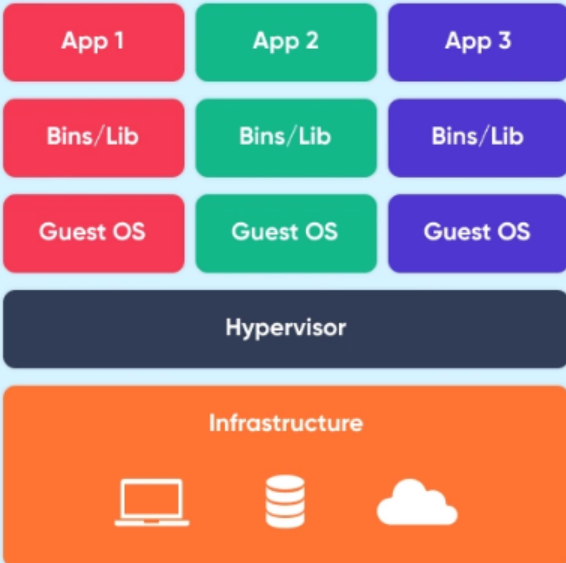
\includegraphics[width=0.4\linewidth]{figures/virtual_machine.png}
    \caption{Structure of vertual machines.}
    \label{fig:Virtual_Machine}
\end{figure}
          \newline
          \textbf{Advantages}
          \begin{itemize}
              \item \textbf{Complete Isolation}: \ac{VMs} operate in total isolation, effectivly wording as independent systems. this isolation ensures that these machine are protected from any harmful exploits, or interference from other \ac{VMs} sharing the same host. While it is still possible for a virtual machine to be vulnerable to some exlpoits, the contaminated virtual machine will not affect the neighboring \ac{VMs} due to this isolation, preventing any cross-contamination amoung virtual machines.
              \item \textbf{Dynamic Development}: \ac{VMs} offer more dynamic development environment. Starting from basic setup, virtual machine can be treated like individual computers. this adaptability enables the direct installation of software, enabling the hands-on development process. Additionally, virtual machines allow for the creating of images, capturing their configurations at any given time.
          \end{itemize}

          \textbf{Disadvantages}
          \begin{itemize}
              \item \textbf{Cost of Storage Space}: It is worth noting that virtual machine take up a lot of space, due to the fact that they virtualize the entire machine. This expansion can lead to potential disk storage issues as the virtual machines keep expanding. Therefor it is crucial to keep monitoring and managing the consumtion to ensure optimal performance and to avoid any disruption on the virtual machine.
              \item \textbf{Speed of Iteration}: Creating and maintaining a virtual machines can be a complex and time-consuming process, as it involves setting up an entire system stack. Modefiying a snapshot of a virtual machine can require significant efforts to rebuild and ensure its expected functionality.
          \end{itemize}
    \item \textbf{Containers}: Containers take an alternative approach, by bunding the application with its necessary binaries, libraries and dependencies into a single package. Unlike traditional techniques, containers mimic the host operating system, giving each container the illusion of being isolated and that it is interactiting with its own virtual kernal, while the truth is, that all containers on host are sharing the same kernal. As demonstrated in \autoref{fig:Containers}. This shared kernal design alloes one \ac{OS} instance to run several isolated containers, making them lightweight and faster to boot compared to virtual machines. This efficiency is resource management and the accelerated application delivery highlights the advantages of containers over \ac{VMs}.
          \begin{figure}[htbp]
    \centering
    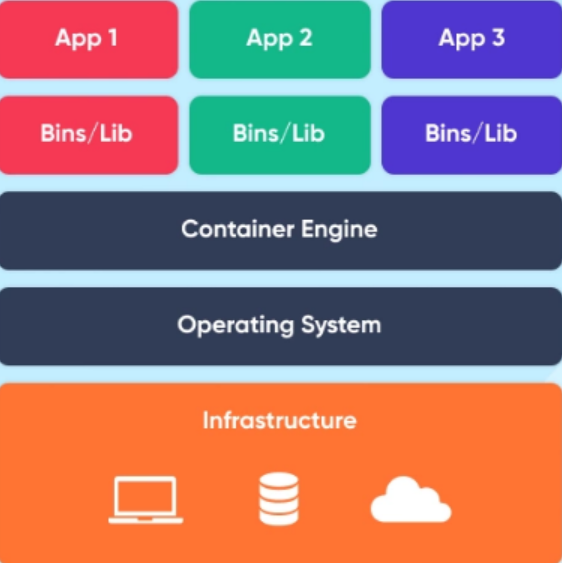
\includegraphics[width=0.445\linewidth]{figures/containers.png}
    \caption{General structure of containers.}
    \label{fig:Containers}
\end{figure}
          \newline
          \textbf{Advantages}
          \begin{itemize}
              \item \textbf{Speed of Iteration}: Due to the fact that containers are lightweight and include only the essential high-level software, as we saw earlier, they possess a remarkable capability for rapid development and iteration. Their basic design and focus on minimalism allow efficient modification capabilities.
              \item \textbf{Robust ecosystem}: Container runtime system offer developers access to pre-defined repositories. These repositories provide an extensive selection of popular software applications, such as databases and messaging systems, that are fast to restore and execute. This setup can help development teams to save time and focus on their core tasks.
          \end{itemize}

          \textbf{Disadvantages}
          \begin{itemize}
              \item \textbf{Shared host exploits}: Containers are built on a shared hardware infrastructure below the operating system layer. That means it is possible that an exploit in one container could break out of the container and affect the hardware that is shared with other containers. This poses a security risk when using one of these public images as they may contain exploits or be vulnerable to being hijacked by nefarious actors.
                    % TODO add one more cons 
          \end{itemize}
\end{enumerate}
\subsection{Docker}
Docker\footnote{https://docs.docker.com/}'\footnote{https://hub.docker.com/} \cite{Intro_Docker} is the leading containerization technology in the market taht provides open-source tools to simplify the creating, deployment, and management of containerized applications. It serves a wide range of users, from open-source enthusiasts to large-scale enterprises with its versatile versions.
\newline
Docker's containerization technology is predicated upon capabilities of the linux kernal, basically exploting mechanisms such as \ac{cgroups} and kernal namespaces, in order to create and manage environments that are somewhat isolated, allowing for efficient resource management.
These \ac{cgroups} are equiped with the capabilities for monitoring and managing resources such as CPU, disk IO, network, and memory for a collection of processes.
Additionally, namespaces play a critical role is ensuring that process groups and resources are isolated from ane another.
In docker, each container is assigned a unique set of namespaces and processes, which allows it to have its own view of the system, including its own network interfaces and file systems.

\subsection{Why Use Docker in Machine Learning}
The lifecycle of machine learning involves a series of steps aimed at leveraging \ac{ML} and \ac{AI} technologies to meet business goals.
This include the initial setting of both business and project-specific goals, acquiring and analyzing relevant data, applying different algorithms to model the data, interpreting the outcomes, and sharing them with stakeholders, and finally deploying and sustaining the project.
Given the rapid pace of technological and market evolution, it is essential to go through multiple iterations and experiments in order to swiftly adapt to the variuos changes and to ensure a seccessful deployment of reliable project that satisfy business expectations \cite{Docker_Archi}.
\newline
Docker encapsulate the entire dependencies of a project down to the host \ac*{OS}. This helps prevent issues,
where projekts function smoothly on one machine and but preforms horribly on another (\autoref{fig:It_Worked_On_My_Machine}).
By using Docker, we are essentially sharing our entire environment rather than just the dependencies and source code.
Doing so, allows for seamless collaboration across machine learning projects while ensuring consistency, portability, and effective dependency management.
Compared to \ac*{VMs} docker is lightweight, which in turn inhances the speed of each iteration and allows for faster deployment of the project.
\begin{figure}[htbp]
    \centering
    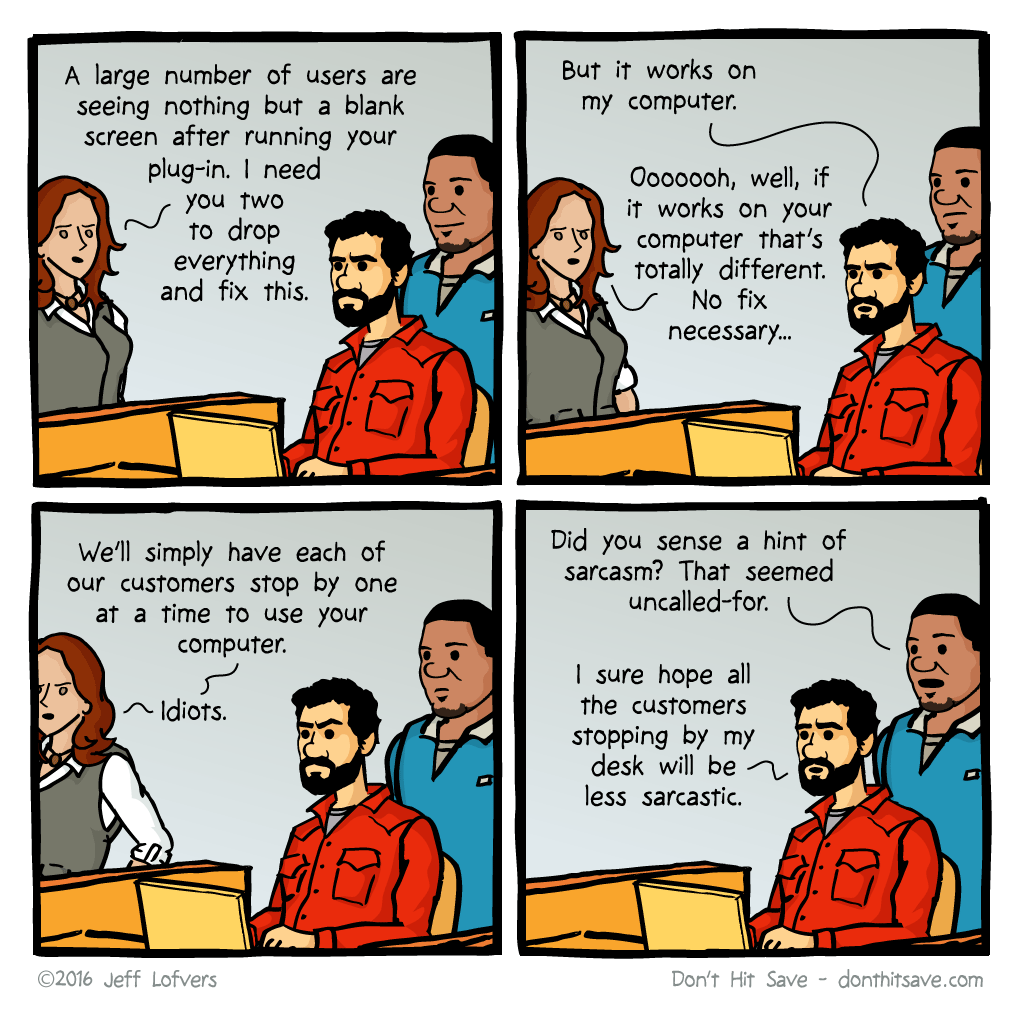
\includegraphics[width=0.4\linewidth]{figures/it-worked-on-my-machine.png}
    \caption{It worked on my machine meme.}
    \label{fig:It_Worked_On_My_Machine}
\end{figure}

\subsection{Usage Scenario}
Before I start showcasing the usage of docker in machine learning, a machine learning project has to be created first. Under this \href{https://github.com/linuxUser10111/thesis}{github repository}\footnote{https://github.com/linuxUser10111/thesis} you can find a \ac{CNN} project that takes a 2D picture of hand-written numbers and tries to prodict the number written on that picture.
The structure of the is as shown in below.
\colorbox{white}{ }
\newline
\colorbox{blue!10}{
    \begin{minipage}{\textwidth}
        \color{RoyalBlue}
        \dirtree{%
            .1 ..
            .2 app.yaml.
            .2 main.py.
            .2 requirements.txt.
            .2 templates.
            .3 homepage.html.
            .3 prediction.html.
            .2 README.md.
        }
        
        \label{dat:Working_Directory_tree}
    \end{minipage}
}
\newline
I used the MNIST library to train the model, which is a dataset of 70,000 images of hand-written numbers. 
The dataset is split into 60,000 training images and 10,000 testing images. 
The model is trained for 50 epochs with a batch size of 512.
\newline
Now that the foundation is set, we can start using docker to encapsulate the project.
% \newline
% https://thinksys.com/devops/docker-components/#:~:text=The%20basic%20components%20include%20Docker,the%20advanced%20components%20of%20Docker.
% First it is important to distinguish between docker components:
% \begin{itemize}
%     \item \textbf{Docker Client}: The docker client is the interface that allows us to interact with the docker daemon. It is the command line interface that we use to create, run, and manage containers. The docker client can be installed on any operating system, including Windows, Linux, and macOS. It is available as a standalone executable or as a package that can be installed through a package manager such as apt or yum. The docker client can be used to manage both local and remote docker daemons. It is also possible to use the docker client to manage multiple docker daemons at once.
%     \item \textbf{Docker Image}: A docker image is a read-only template that contains all the necessary instructions and dependencies to create a docker container. It is essentially a snapshot of a docker container that can be used to create new containers. Docker images are built using a dockerfile, which is a text file that contains a set of instructions for building the image. These instructions can include commands for installing software, copying files, and setting up environment variables. Docker images can be stored in a docker registry, which is a centralized repository for docker images. This allows developers to share and reuse docker images, making it easier to create and manage containers.
%     \item \textbf{Docker Daemon}: The docker daemon is the background service that manages docker containers. It is responsible for creating and running containers, managing resources, and communicating with the docker client. The docker daemon can be installed on any operating system, including Windows, Linux, and macOS. It is available as a standalone executable or as a package that can be installed through a package manager such as apt or yum. The docker daemon can be configured to run in the background as a system service or as a standalone process. It can also be configured to run on a remote server, allowing developers to manage containers remotely.
% \end{itemize}

%% adding a new page to seperate this two sections (for now)
\newpage

\section{Hybrid Approaches}

\section{Cloud Execution}